
\subsection*{\textbf{Question 5.e)}}
\begin{quote}

\textbf{Problem}
\begin{quote}
Generalize your own FFT algorithm to 2 and 3 dimensions and make a plot of the FFT of a 2D function (no bivariate Gaussian) and compare it with the analytical FFT of your FFT. Also make a plot of the FFT of a 3D multivariate Gaussian function, plot 3 slices centered at the center for the 3 different slice options x-y, x-z,y-z.
\end{quote}

\textbf{Solution} 
\begin{quote}

The code for the 2D and 3D implementation makes use of the code for the 1D implementation. In 2D the FFT is first taken over the first axis of the input matrix and then over the second axis. In 3D the FFT2 is first taken over the first axis and then the FFT is taken over the third axis. 
The code is not generalized to N-dimensions, as the question did not ask to write your own swapaxis algorithm. 
\\
The chosen function to 2D fourier transform is $\cos(x+y)$. The analytical result consists of two 2D delta functions. The code that makes the plots for the 2D FFT and the 3D FFT can be found below, the implementation its self can be found on page 75. The plots can be found below the code.
\end{quote}
\newpage

\textbf{Code - Plot}
\begin{quote}
The code that creates the plots.
%The code that creates the slices, cell 0 and cell 4 in a 3D grid of size 16.
\lstinputlisting[firstline = 162, lastline=231]{./Code/assigment_5.py}
\end{quote}

\textbf{Plot - 2D}\\
\begin{quote}

\begin{figure}[!ht]
\centering
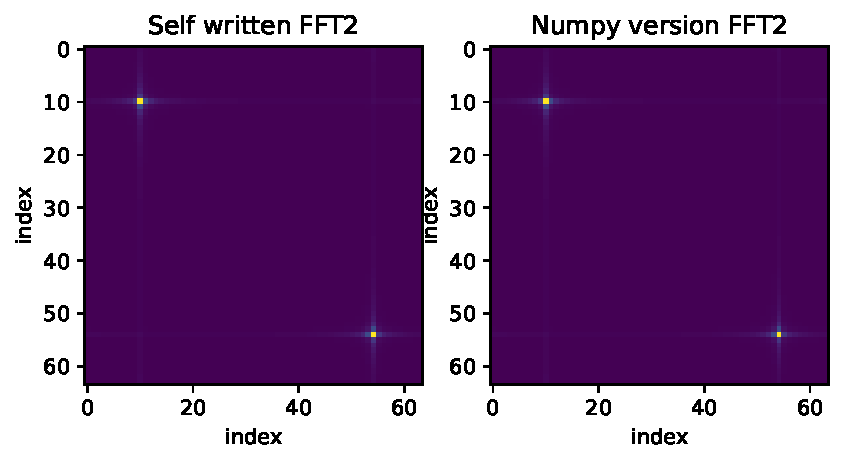
\includegraphics[width=15cm, height=7.5cm]{./Plots/5e_2d_fft.pdf}

\caption{The 2D fourier transformation for the function $\cos(x+y)$. Left, the own implementation of the FFT2 (left) and right the numpy implementation. The results show that the self written version appears to be equal to the numpy version. For the cosine two delta peaks are expected to arise which can also be seen. The peaks are not infinite sharp as that would require an infinite amount of samples. }
\end{figure}
\end{quote}
\textbf{Plot - 3D}
\begin{quote}
\vspace*{-0.5cm}

\begin{figure}[!hb]
\centering
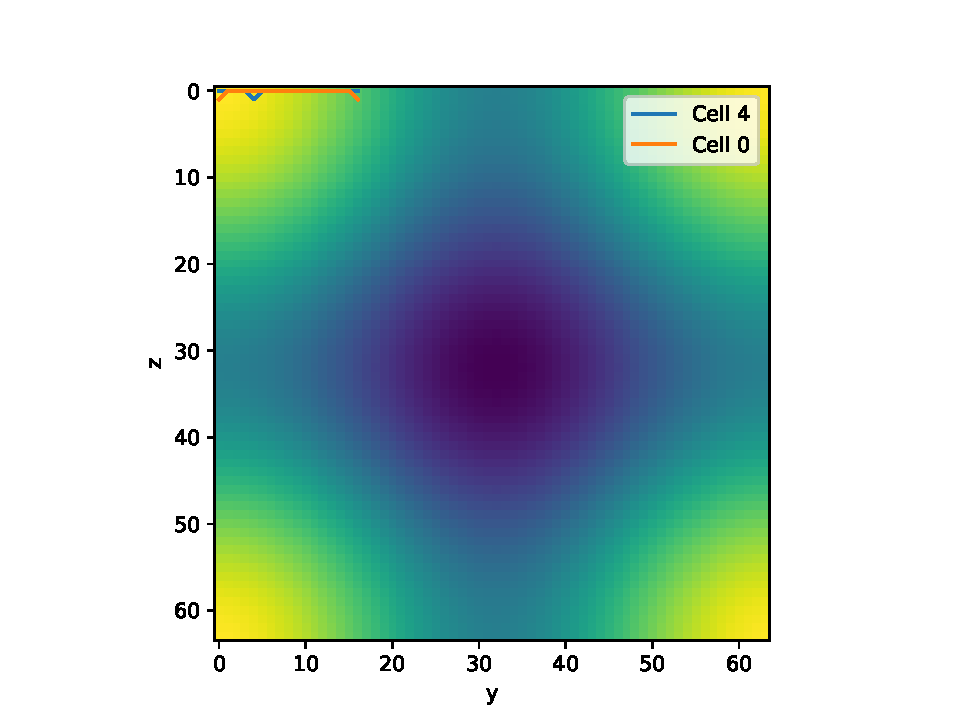
\includegraphics[width=14cm, height=7.5cm]{./Plots/5e_gaussian_yz.pdf}
\caption{The yz slice around the center of the 3D Fourier transform of a multivariate gaussian with $\mu = 0$ and $\sigma = 0.5$.  The slice should be perfectly symmetric and the result shows that this is indeed the case. }
\end{figure}
\newpage

\begin{figure}[!ht]
\centering
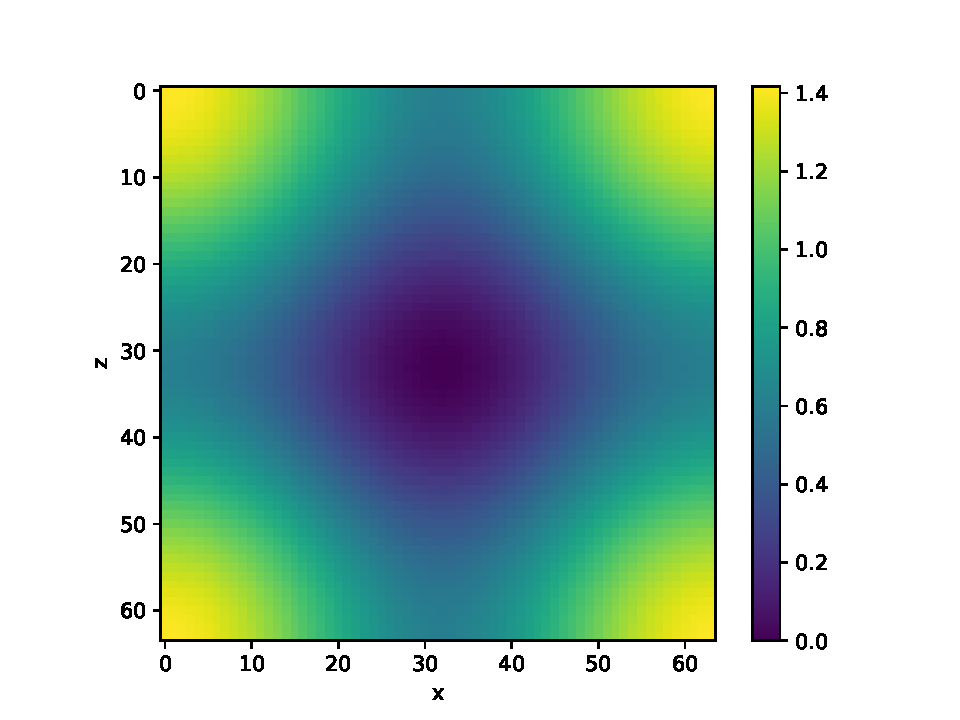
\includegraphics[width=14cm, height=7.5cm]{./Plots/5e_gaussian_xz.pdf}
\caption{The xz slice around the center of the 3D Fourier transform of a multivariate gaussian with $\mu = 0$ and $\sigma = 0.5$.  The slice should be perfectly symmetric and the result shows that this is indeed the case. }
\end{figure}

\begin{figure}[!hb]
\centering
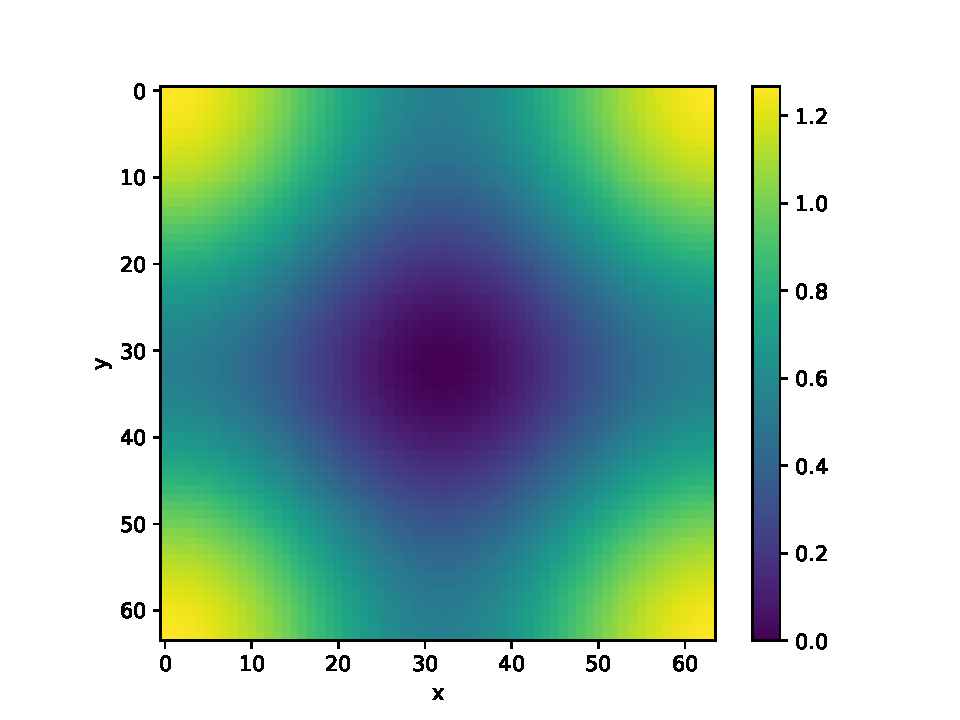
\includegraphics[width=14cm, height=7.5cm]{./Plots/5e_gaussian_xy.pdf}
\caption{The xy slice around the center of the 3D Fourier transform of a multivariate gaussian with $\mu = 0$ and $\sigma = 0.5$.  The slice should be perfectly symmetric and the result shows that this is indeed the case. }
\end{figure}
\end{quote}

\end{quote}

%\end{quote}












